\section{Features of the \openshmem Analyzer}
\label{chapter:features}

\subsection{Overview}

The \openshmem Analyzer will generate an HTML file file with the
callgraph of a program that can be related to the source code via HTML
links. In addition the main HTML file contains a list of warning
messages generated by the tool and that can be related to the source
code via HTML links.

The following command opens the HTML file that contains the callgraph
and the error messages of the program (based on the previous example)

\begin{lstlisting}[language=bash]
  $ firefox myprogram.html
\end{lstlisting}

(Or use any web browser of your choice.)

\subsubsection{Callgraph}

The call graph gives the structure of the program, where there is a
node for each procedure in the program and a directed edge links a
pair of nodes if and only if the procedure corresponding to the source
node may invoke the sink node's procedure at run time. If you click on
a node, the source text of the corresponding procedure will be
displayed in the HTML browser. The edges of the graph represent the
different callsites where the procedures are invoked. The user can
click on the edges to relate them to the source code. The callgraph
nodes are colored in the following format:

\vspace{0.1in}

\begin{center}
  \begin{tabular}{| p{10cm} | l |}
    \hline
    Procedures containing \openshmem calls & \textcolor{LightBlue}{light blue} \\
    \hline
    Procedures not containing \openshmem calls & \textcolor{Silver}{silver} \\
    \hline
    Procedures representing \openshmem & \textcolor{Pink}{pink} \\
    \hline
  \end{tabular}
\end{center}

\vspace{0.1in}

For the edges, callsites to \openshmem are colored:

\vspace{0.1in}

\begin{center}
  \begin{tabular}{| p{10cm} | l |}
    \hline
    I/O operations (i.e.\ puts, gets) & \textcolor{Blue}{blue} \\
    \hline
    Reductions & \textcolor{Purple}{purple} \\
    \hline
    Broadcasts & \textcolor{Red}{red} \\
    \hline
    Atomics & \textcolor{Orange}{orange} \\
    \hline
    Memory management calls (i.e.\ dynamic allocation / deallocation of symmetric memory) & \textcolor{Yellow}{yellow} \\
    \hline
    State calls (i.e.\ num\_pes, my\_pe) & \textcolor{Green}{green} \\
    \hline
    Synchronization calls & \textcolor{Red}{red} \\
    \hline
  \end{tabular}
\end{center}

\vspace{0.1in}

Figure~\ref{fig:is-callgraph} shows a portion of a callgraph generated
for the IS NAS Parallel Benchmark:

\begin{figure}[!ht]
  \begin{center}
    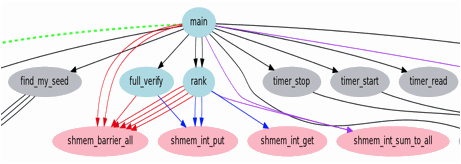
\includegraphics[width=0.8\textwidth]{./image004}
    \caption{The \openshmem callgraph of the IS NAS parallel benchmark}
    \label{fig:is-callgraph}
  \end{center}
\end{figure}

In addition to the callgraph, the color legend for the nodes and edges
is displayed in figure~\ref{fig:colors}

\vspace{0.1in}

\begin{figure}[!ht]
  \begin{center}
    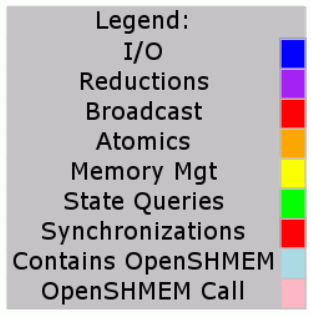
\includegraphics[width=0.25\textwidth]{./osa_color_legend}
    \caption{The color legend for the callgraph of an \openshmem program}
    \label{fig:colors}
  \end{center}
\end{figure}

When a node or a callsite is clicked, the browser will display the
corresponding source code with highlight syntax formatted in HTML, as
in figure~\ref{fig:app-source}.

\vspace{0.1in}

\begin{figure}[!ht]
  \begin{center}
    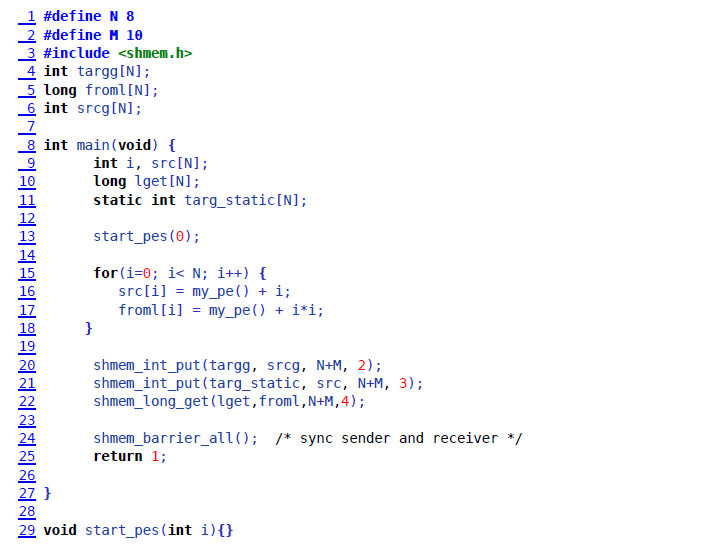
\includegraphics[width=0.8\textwidth]{./source_listing_test_bounds}
    \caption{Application source code as displayed in the browser}
    \label{fig:app-source}
  \end{center}
\end{figure}

\subsection{Displaying the \openshmem Analyzer Warnings}

The \openshmem Analyzer is able to display \openshmem warning messages
together with the callgraph. The warning messages are also displayed
when the tool is invoked at command line. When the warning messages
are displayed with the callgraph, each message contains an HTML link
that relates the message to the source. Figure~\ref{fig:warnings} is
an example of how the \openshmem Analyzer displays its warning messages
together with the source code.

\vspace{0.1in}

\begin{figure}[!ht]
  \begin{center}
    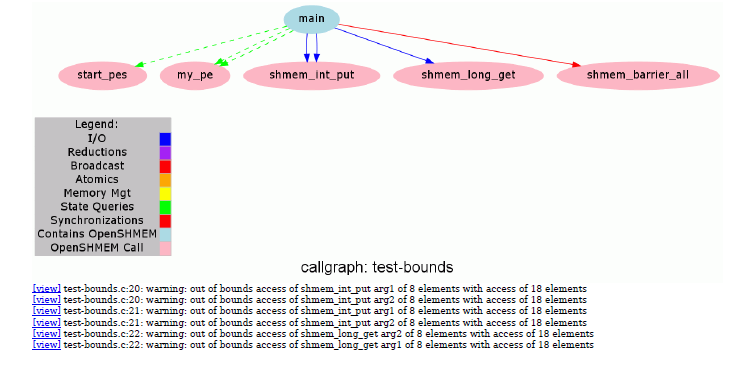
\includegraphics[width=1.0\textwidth]{./callgraph_test_bounds}
    \caption{Callgraph with the \openshmem Analyzer warning messages.
      The warning message contains a link to the source code}
    \label{fig:warnings}
  \end{center}
\end{figure}

The messages contain the line number and the source file name of the
\openshmem call that is triggering the warning.

\begin{minipage}{\linewidth}

  \subsection{Analysis available in the \openshmem Analyzer}

  The \openshmem Analyzer is able to perform the following analyses:

  \vspace{0.1in}

  \begin{itemize}
  \item check the ordering of \openshmem initialization and
    finalization calls;
  \item check if there is an \openshmem initialization call in the
    program;
  \item check if there is more than one \openshmem initialization
    call;
  \item check if \openshmem calls are using symmetric memory variables;
  \item check for out-of-bounds access for arrays in \openshmem calls;
  \item check for out-of-bounds strided access of arrays;
  \item check if one of the arguments of the \openshmem calls
    evaluates to NULL;
  \item perform constant propagation and common sub-expression
    elimination to simplify the arguments of an \openshmem call. This
    is useful to check if some arguments evaluate to constants or to
    simplify the analysis and accuracy of the tool;
  \item check if pointers to symmetric data are allocated with
    shmalloc calls;
  \item check if any variables used in expression for pointer
    arithmetic of symmetric variables are initialized;
  \item check if global pointers to symmetric data are initialized;
  \item check if pointers to symmetric data are aliased with other
    pointers that can have side-effects to the \openshmem call;
  \item check if the \openshmem calls arguments are of the correct
    types or storage allocation for \openshmem typeless calls.

  \end{itemize}

\end{minipage}

\subsection{The \openshmem Analyzer Warning Messages}

The following shows examples of warning messages output by the tool

\vspace{0.2in}

\begin{minipage}{\linewidth}
\subsubsection{Multiple \openshmem initialization calls}

\begin{lstlisting}[language=OSH+C]
  int main(...)  {                void sub (...) {
      ...                             ...
      start_pes();                    start_pes();       
      sub(...);                   } 
  }
\end{lstlisting}
\begin{alltt}
  warning: more than one \openshmem initialization call found
\end{alltt}
\end{minipage}

\vspace{0.2in}

\begin{minipage}{\linewidth}
\subsubsection{Non-symmetric variable used in \openshmem call}

\begin{lstlisting}[language=OSH+C]
  int sub(...) {
    long target, source;
    ...
    shmem_long_get(target, source, ...);
  }
\end{lstlisting}
\begin{alltt}
  badget.c:65: warning: non-symmetric variable in arg2 of shmem_long_get
\end{alltt}
\end{minipage}

\vspace{0.2in}

\begin{minipage}{\linewidth}
\subsubsection{Out-of-bounds accesses in \openshmem call}

\begin{lstlisting}[language=OSH+C]
  #define N 8
  #define M 8

  int sub (...) {
    ...
    static int targ[N], src[N];
    ...
    shmem_int_put(targ, src, N + M, 2);
    ...
  }
\end{lstlisting}
\begin{alltt}
  test-bounds.c:20: warning: out of bounds access of shmem_int_put arg1 of 8
  elements
\end{alltt}
\end{minipage}

\vspace{0.2in}

\begin{minipage}{\linewidth}
\subsubsection{Out-of-bounds accesses in \openshmem call determined with constant propagation (must use -O3)}

\begin{lstlisting}[language=OSH+C]
  #define N 8
  #define M 8

  int sub (...) {
    int len = N;
    static int targ[N], src[N];
    ...
    for(i = 0; i < M; i++) len++;
    ...
    shmem_int_put(targ, src, len, 2);
    ...
  }     
\end{lstlisting}
\begin{alltt}
  test-bounds-constprog.c:23: warning: out of bounds access of shmem_int_put
  arg1 of 8 elements with access of 16 elements
\end{alltt}
\end{minipage}

\vspace{0.2in}

\begin{minipage}{\linewidth}
\subsubsection{Out-of-bounds accesses in \openshmem call with strided access}

\begin{lstlisting}[language=OSH+C]
  int src2[N];
  ...
  int sub(...) {
    ...
    shmem_iget32(dest2, src2, 1, 2, N, npes - 1);
    ...
  }
\end{lstlisting}
\begin{alltt}
  test_shmem_get_globals.c:297: warning: out of bounds access of shmem_iget32
  arg2 of 7 elements with access of 14 elements
\end{alltt}
\end{minipage}

\vspace{0.2in}

\begin{minipage}{\linewidth}
\subsubsection{Pointer is initialized with the wrong memory allocator (non-symmetric)}

\begin{lstlisting}[language=OSH+C]
  int sub(...) {
    ...
    float *y;
    ...
    y = (float *) malloc((n_local1 - n_local0 + 2) * sizeof(float));
    ...
    shmem_float_put(&y[n_local0-1+1], &y[n_local1-1], 1, _my_pe() + 1);
    ...
  } 
\end{lstlisting}
\begin{alltt}
  shmem_heap.c:35: warning: variable arg1 of call shmem_float_put is
  initialized with malloc
\end{alltt}
\end{minipage}

\vspace{0.2in}

\begin{minipage}{\linewidth}
\subsubsection{Global Pointer is not initialized}

\begin{lstlisting}[language=OSH+C]
  float *y;

  int sub(...) {
    ...
    shmem_float_put(&y[n_local0-1+1], &y[n_local1-1], 1, _my_pe() + 1);
    ...
  }
\end{lstlisting}
\begin{alltt}
  shmem_heap-global.c:20: warning: global variable arg1 of call shmem_float_put
  is uninitialized
\end{alltt}
\end{minipage}

\vspace{0.2in}

\begin{minipage}{\linewidth}
\subsubsection{Wrong storage type for typeless \openshmem call}

\begin{lstlisting}[language=OSH+C]
  long lfrom;

  int sub(void) {
    ...
    shmem_get32(lget, lfrom, N, 4);
    ...
  }
\end{lstlisting}
\begin{alltt}
  test-types.c:23: warning: wrong storage class of shmem_get32 arg2 of 8 bytes
\end{alltt}
\end{minipage}

% \vspace{0.2in}
% 
% \begin{minipage}{\linewidth}
% \subsubsection{Symmetric variable in the \openshmem call may be aliased with a pointer}
% 
% \begin{lstlisting}[language=OSH+C]
%   int sub(...) {
%     ...
%   }
% \end{lstlisting}
% \begin{alltt}
%   1_put_afteruse_g.c:37: warning: Symmmetric Variable named y in arg1 of
%   \openshmem call
% \end{alltt}
% \end{minipage}
